\documentclass[17pt]{beamer}
\usetheme{Boadilla}
\usepackage{graphicx}
\usepackage{algorithm2e}
\graphicspath{{images/}}
\title{CMPT 155: Computer Applications for Life Sciences}
\subtitle{Lecture 1: Syllabus and Introduction to Excel}
\author{Ivan E. Perez}
\institute{}
\date{\today}
\usepackage{booktabs} % Allows the use of \toprule, 
\usepackage{appendix}
\usepackage{enumerate,multicol}
\usepackage{amsmath, amssymb, amsthm}
\usepackage{tikz}

\begin{document}
	\begin{frame}
		\titlepage
	\end{frame}
	
	\begin{frame}
		\frametitle{Presentation Outline}
		\tableofcontents
	
	\end{frame}
	
	\section{Syllabus and Course Introduction}
	\begin{frame}
		\frametitle{General Info}
		\begin{itemize}
			\item Email: iperez04@manhataan.edu
			\item Office: RLC 204
			\item Office Hours: Friday 10am-12pm
			\item Website: \color{blue}{\href{https://ivaneperez.com/teaching/CMPT155/}{https://ivaneperez.com/teaching/CMPT155/}}
		\end{itemize} 
	\end{frame}
	\begin{frame}
		\frametitle{About the Course}
		\begin{itemize}
			\item Section 01: Tuesday, Wednesday Friday 8:00-8:50 AM
			\item Section 02: Tuesday, Wednesday, Friday 9:00 - 9:50 AM
		\end{itemize}
	\end{frame}
	\begin{frame}
		\frametitle{Textbook}
		\begin{itemize}
			\item \underline{Computer Application for Life Sciences},
			Revised edition, Joan Harnett, Linus Learning, 2014.
			\item ISBN 13: 978-1-60797-501-4
		\end{itemize}
	\bigskip
		
\includegraphics[width=25mm]{Computer-Applications-for-Life-Sciences.jpg}
	\end{frame}
\begin{frame}
	\frametitle{Grading}
		\begin{itemize}
			\item $1^\text{st}$ Midterm Exam: 15\%
			\item $2^\text{nd}$ Midterm Exam: 15\%
			\item Final Exam: 30\%
			\item Attendance \& Participation: 5\% 
			\item Lab Assignments and Homework: 35\%
		\end{itemize}
\end{frame}
\begin{frame}
	\frametitle{Important Dates}
	\begin{itemize}
		\item \textit{Tentative} Date of 1st Midterm Exam: 10/01/2021 
		\item Midterm Grades Due: 10/19/2021
		\item \textit{Tentative} Date of 2nd Midterm: 11/05/2021 
		\item Last Day to Withdraw from Courses: 11/19/2021
		\item Date of Final Exam: 12/17/2021
	\end{itemize}
\end{frame}
\begin{frame}
	\frametitle{Attendance Policy}
	\begin{itemize}
		\item \textbf{Attendance is Mandatory}
		\item Attendance and \textbf{Participation} counts for 5\% of your grade.
	\end{itemize}
What is Participation?
\begin{enumerate}
	\item Engaging with the class
	\item Asking questions
	\item participating in the moodle forum
\end{enumerate}
\end{frame}
\begin{frame}
	\frametitle{Electronic Devices}
	\begin{itemize}
		\item Do not Check e-email or visit websites extraneous to the course during class.
		\item Phones should be silent(including rumble) in 2021. 
	\end{itemize}
\end{frame}
\begin{frame}
	\frametitle{Homework Policy}
	\begin{itemize}
		\item Submit Homework Assignments on Moodle.
		\item Due 1 week after announced ()Typically on Fridays). 
		\item \textbf{\color{red}{No Late Work is Accepted}}
		\item Assignments can be worked out together, but must be typed separately.
	\end{itemize}

Advice for computer/programming based homework:
\begin{enumerate}
	\item Isolate the ideas/chapters of the course material are explored in the assignment.
	\item Give it an honest try,find problems and issues to take note of.
	\item \textbf{Give yourself time to be confused}. 
	\item Try again at a later date.  
\end{enumerate}
\end{frame}
\begin{frame}
	\frametitle{Advice to be Sucessful in this Course}
	\begin{itemize}
		\item Attend Class
		\item Take notes
		\item \textbf{Engage with the Material} by doing examples.
		\item Ask Questions!
		\item Save/Document programs.
		\item Do personal programs and projects! (e.g., Tracking Spending, Budgeting, Fitness goals)
	\end{itemize}
\end{frame}
\section{Introduction to Excel}
\begin{frame}
	\frametitle{About Excel}
	\begin{itemize}
	\item It's not free
	\item Free options
	\begin{enumerate}
		\item Campus computers
		\item RLC 103 8am-10pm
		\item library 24h 
		\item Open-Source! LibreOffice! 
	\end{enumerate}
	\end{itemize}
\end{frame}
\begin{frame}
	\frametitle{About Excel Cont.}
	\begin{itemize}
		\item Excel is a Front-End Data Manipulation software, for the Language Visual Basic
		\item Excel is can store smallish ($<1$GB) datasets.
	\end{itemize}	
\end{frame}
\begin{frame}
	\frametitle{Common Spreadsheets}
	\begin{itemize}
		\item Business Documents
		\begin{itemize}
			\item financial statements, invoices,expense reports.		
		\end{itemize}
		\item Personal Documents
			\begin{itemize}
				\item Budgets, Chore/Bill Split		
			\end{itemize}
		\item Business Documents
			\begin{itemize}
				\item Numerical Data, Simulated data, Quantitative/Qualitative data.   
			\end{itemize}
	\item Excel is great because: it 
	\begin{itemize}
		\item Portable way to share/collaborate on data analysis.
		\item Easy to follow/traceable methods of visualizing data, following data manipulation.
		\item Templates are easy to make and distribute. 
	\end{itemize}
	\end{itemize}
\end{frame}
\begin{frame}
	\frametitle{Ex:Annual Cancer Deaths}
		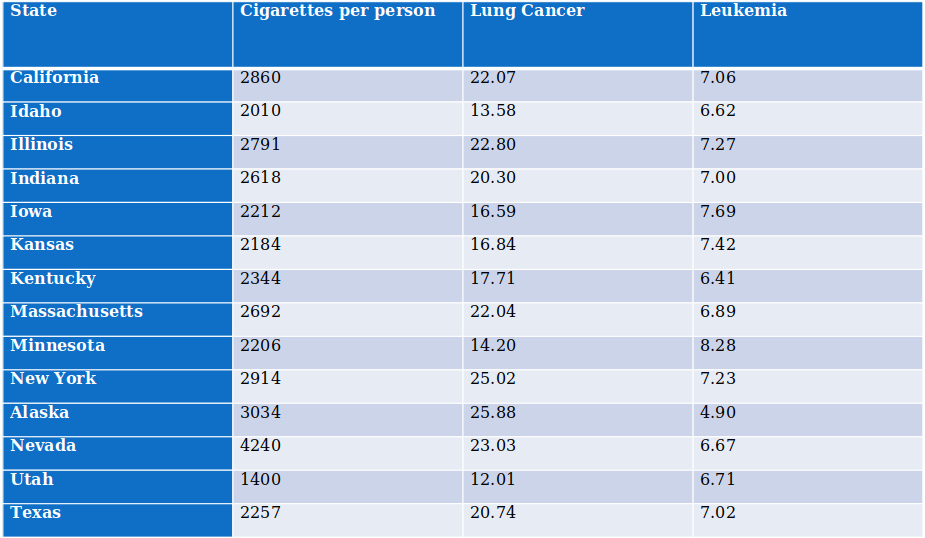
\includegraphics[width=\linewidth]{cancerdeathper100k}
\end{frame}
\begin{frame}
	\frametitle{}
\end{frame}
\end{document}





